\documentclass[tikz,border=12pt]{standalone}
\usepackage[T1]{fontenc}
\usepackage{mathpazo}
\usepackage{amsmath,amssymb}
\usetikzlibrary{arrows.meta, positioning, calc}

\definecolor{stblue}{HTML}{7B97AD}
\definecolor{rwgold}{HTML}{B8995E}
\definecolor{sage}{HTML}{7A9A7E}
\definecolor{dkbrown}{HTML}{3D3530}
\definecolor{wmgray}{HTML}{7B7067}
\definecolor{cream}{HTML}{F9F6F0}
\definecolor{border}{HTML}{D4C9B8}
\definecolor{terracotta}{HTML}{C47A6A}
\definecolor{lavender}{HTML}{907EA0}

\begin{document}
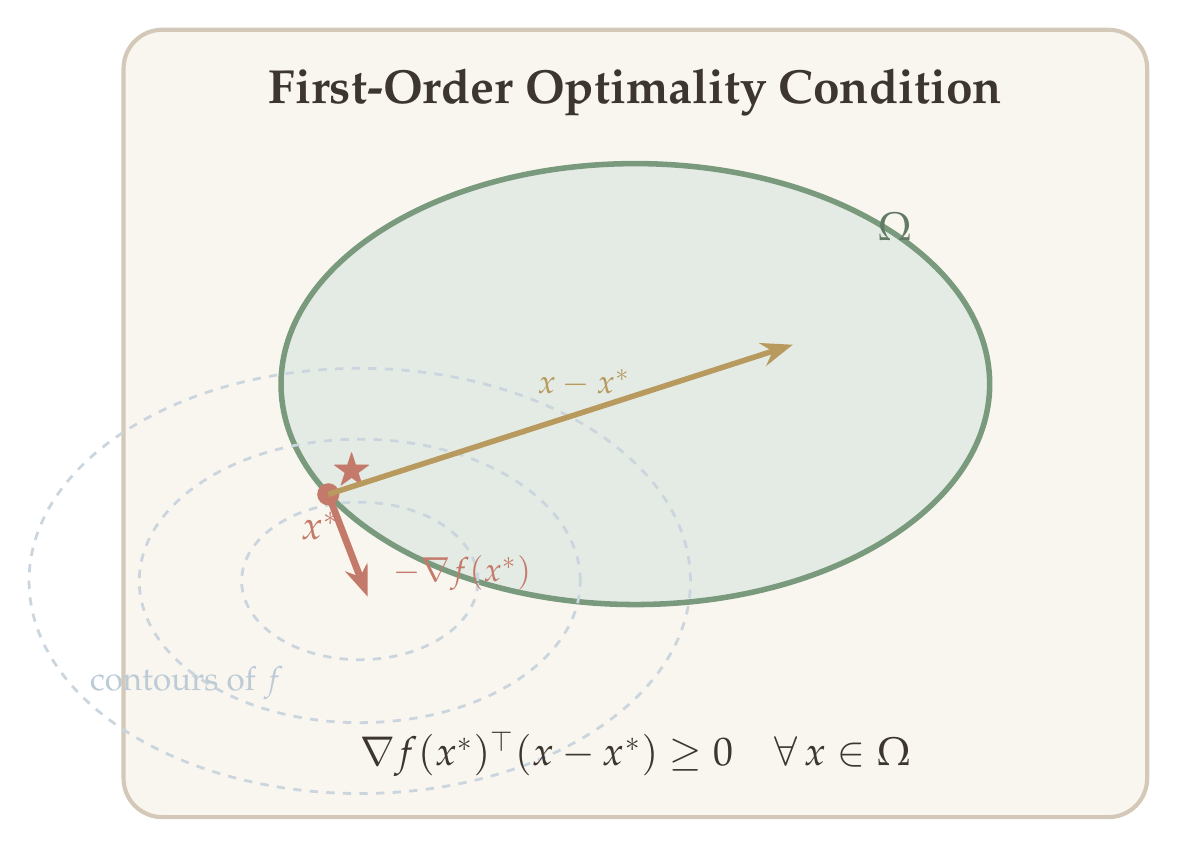
\begin{tikzpicture}[>={Stealth[length=4mm, width=3mm]}]

% Background
\fill[cream, rounded corners=14pt] (-1.0,-1.5) rectangle (12.0,8.5);
\draw[border, line width=1.5pt, rounded corners=14pt] (-1.0,-1.5) rectangle (12.0,8.5);

% Title
\node[text=dkbrown, font=\LARGE\bfseries] at (5.5,7.7) {First-Order Optimality Condition};

% Feasible set Omega (ellipse, sage)
\fill[sage!20] (5.5,4.0) ellipse (4.5cm and 2.8cm);
\draw[sage, line width=2pt] (5.5,4.0) ellipse (4.5cm and 2.8cm);
\node[text=sage!80!black, font=\Large\bfseries] at (8.8,6.0) {$\Omega$};

% Contour lines (ellipses centered below-left, level sets of f)
% The unconstrained min is outside Omega at roughly (2.0, 1.5)
\draw[stblue!40, line width=1pt, dashed] (2.0,1.5) ellipse (1.5cm and 1.0cm);
\draw[stblue!40, line width=1pt, dashed] (2.0,1.5) ellipse (2.8cm and 1.8cm);
\draw[stblue!40, line width=1pt, dashed] (2.0,1.5) ellipse (4.2cm and 2.7cm);
\node[text=stblue!50, font=\large] at (-0.2,0.2) {contours of $f$};

% x* is on the boundary of Omega, at the bottom-left where the contour
% is tangent to the feasible boundary.
% Omega ellipse: center (5.5,4.0), a=4.5, b=2.8
% Parametric: x = 5.5 + 4.5*cos(t), y = 4.0 + 2.8*sin(t)
% At t = -120 deg (210 deg): cos(210)=-0.866, sin(210)=-0.5
% x = 5.5 + 4.5*(-0.866) = 5.5 - 3.9 = 1.6
% y = 4.0 + 2.8*(-0.5) = 4.0 - 1.4 = 2.6
% That's on the lower-left of the boundary, good.
\coordinate (xstar) at (1.6,2.6);
\fill[terracotta] (xstar) circle (4pt);
\node[text=terracotta, font=\Large\bfseries] at ($(xstar)+(-0.1,-0.4)$) {$x^*$};

% Star marker
\node[text=terracotta, font=\Large] at ($(xstar)+(0.3,0.3)$) {$\bigstar$};

% Gradient direction: nabla f points away from unconstrained min (toward lower-left)
% So -nabla f points toward unconstrained min (upper-left is wrong; toward (2.0,1.5))
% Actually nabla f at x* points outward from contour center, so from (2.0,1.5) toward (1.6,2.6)
% direction = (1.6-2.0, 2.6-1.5) = (-0.4, 1.1), normalized ~ (-0.34, 0.94)
% -nabla f points toward (2.0,1.5): direction (0.34, -0.94)
% But for the figure we want -nabla f pointing INTO Omega (the gradient condition)
% nabla f points outward from level set center: from (2.0,1.5) toward x*
% So nabla f direction at x* ~ (-0.4, 1.1) normalized
% -nabla f direction ~ (0.4, -1.1) — pointing down-right, away from Omega interior
% Actually no: nabla f at boundary of Omega should point roughly away from Omega interior
% to make the optimality condition meaningful.
%
% Let's think again: f decreases toward its unconstrained min at (2.0, 1.5).
% At x* on Omega boundary, nabla f points away from (2.0,1.5), i.e., outward.
% -nabla f points toward (2.0,1.5), i.e., outside Omega.
% The optimality condition says: for all feasible x, (x - x*)^T nabla f(x*) >= 0
% i.e., all feasible directions make obtuse angle with -nabla f.
% So -nabla f should point outside Omega. Let's draw it.

% -nabla f(x*): points toward the unconstrained minimum (outside Omega)
\draw[terracotta, line width=2.5pt, ->] (xstar) -- ++(0.5,-1.3);
\node[text=terracotta, font=\large] at ($(xstar)+(1.7,-1.0)$) {$-\nabla f(x^*)$};

% A feasible point x inside Omega
\coordinate (xtest) at (7.5,4.5);
\draw[rwgold, line width=2pt, ->] (xstar) -- (xtest);
\node[text=rwgold, font=\large, above=2pt] at ($(xstar)!0.55!(xtest)$) {$x - x^*$};

% Angle arc between -nabla f and feasible direction (obtuse angle)
% -nabla f direction angle: atan2(-1.3, 0.5) ~ -69 deg ~ 291 deg
% feasible direction angle: atan2(4.5-2.6, 7.5-1.6) = atan2(1.9, 5.9) ~ 17.8 deg
% Angle from -nabla f to feasible = 17.8 - 291 + 360 = 86.8 going counterclockwise
% Or from feasible to -nabla f = 291 - 17.8 = 273.2 deg
% The angle between them is about 97 degrees (obtuse, good!)

% Key condition label
\node[text=dkbrown, font=\Large, align=center] at (5.5,-0.7)
  {$\nabla f(x^*)^\top (x - x^*) \geq 0 \quad \forall\, x \in \Omega$};

\end{tikzpicture}
\end{document}
